\chapter{The Shield}
\label{the_shield}
The first step of designing the hardware is determining how to detect when the user is drumming. The two overall methods considered are, force sensitive resistors or simple buttons. They both have some pros and cons. 

Buttons output a simple HIGH/LOW signal making them easy to work with. On the other hand they are bulky and make a clicking noise when pressed.
FSRs can be used to output an analog signal, affording many more types of interactions, if utilizing light and heavy presses. They are also much thinner, making them fit more easily into the glove without being obvious or bulky. They do however require a few extra components to be used properly. Several types of FSRs were available the FSR-151 was chosen as the size and shape made it easy to mount in the glove without being too hard to actually press when finger-drumming.
\blankline 
Lastly an Arduino Uno is used to facilitate communication between the sensors and the computer for the prototype. 

\section{Electronics}
\label{electronics}
The finger drums prototype will consist of 5 FSR-151s connected to analog pins 0 to 4 of an Arduino Uno. In order to get the desired output signal from the FSRs they have to be connected with a normal resistor to create a voltage divider as seen in \autoref{fig:simple_voltage_divider}. 

\begin{figure}[H]
\centering
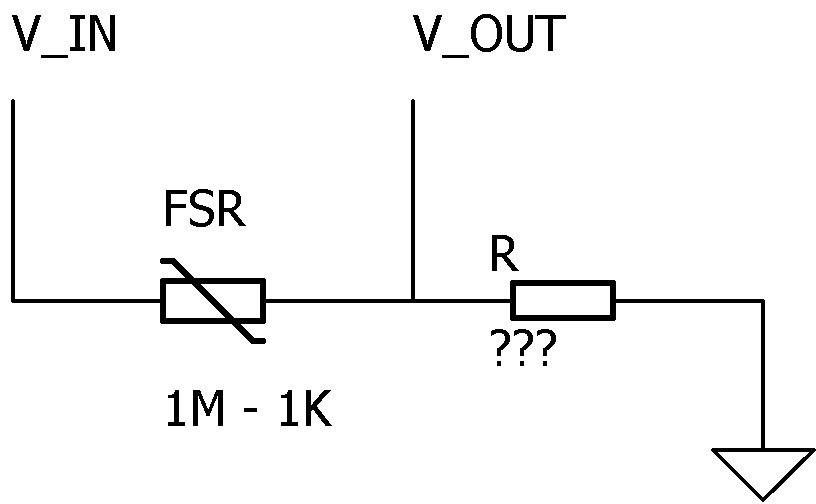
\includegraphics[scale=1.5]{Figure/simple_voltage_divider.png}
\caption{Simple voltage divider with the FSR represented as a variable resistor. }
\label{fig:simple_voltage_divider}
\end{figure}

In order to find a fitting value for the resistor R the formula for a voltage divider is used, \autoref{fig:VoltageDividerFormula}.
\begin{figure}[H]
\centering
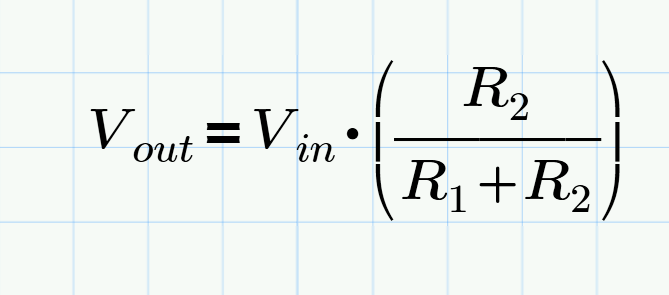
\includegraphics[scale=0.15]{Figure/VoltageDividerFormula.png}
\caption{General formula for a voltage divider.}
\label{fig:VoltageDividerFormula}
\end{figure}

The input voltage, V\textsubscript{in}, is 5V, coming from the Arduino. R\textsubscript{1}, the FSR-151, varies in the range 1 M$\Omega$ to 1 K$\Omega$, depending on the force applied to it, according to the datasheet and follows the curve shown in \autoref{fig:DatasheetCurve}. The ideal output signal is around 0V and 5V depending on the value of the FSR. In \autoref{fig:FinalFormula} the formula is shown with a resistor of 100 k$\Omega$ the output voltage, V\textsubscript{out} will then range from 0.455V to 4.95V, which is close enough to the target output voltage range. 
\begin{figure}[H]
\centering
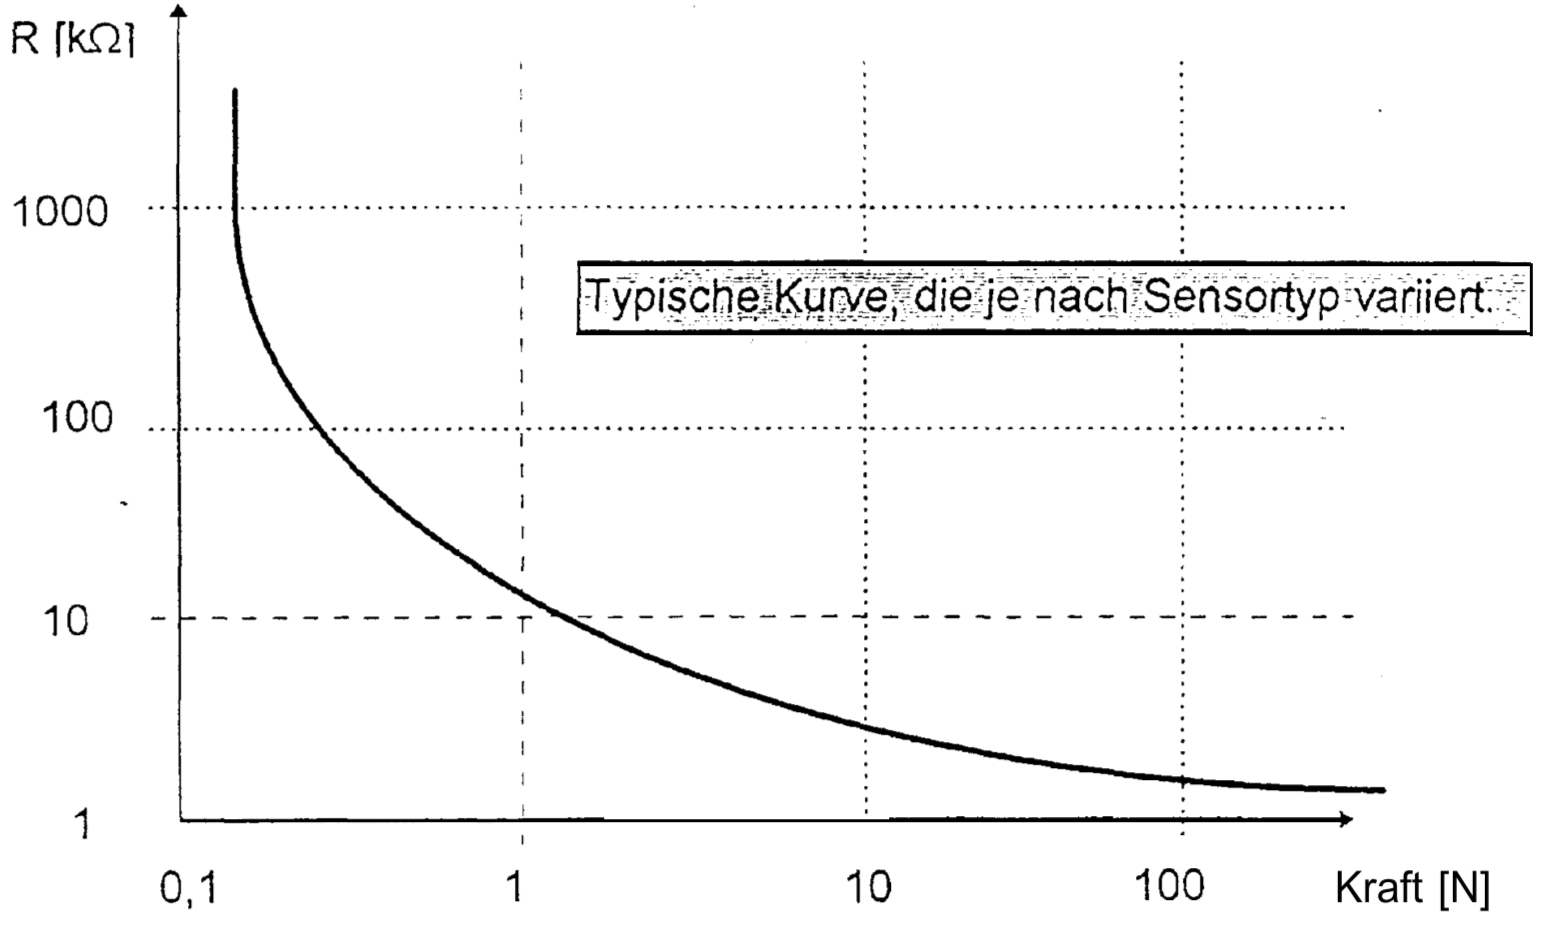
\includegraphics[scale=0.15]{Figure/DatasheetCurve.png}
\caption{The characteristic curve from the FSR-151 datasheet. The X-axis is the force applied in Newton, Y-axis is the resistance in k$\Omega$.}
\label{fig:DatasheetCurve}
\end{figure}

\begin{figure}[H]
\centering
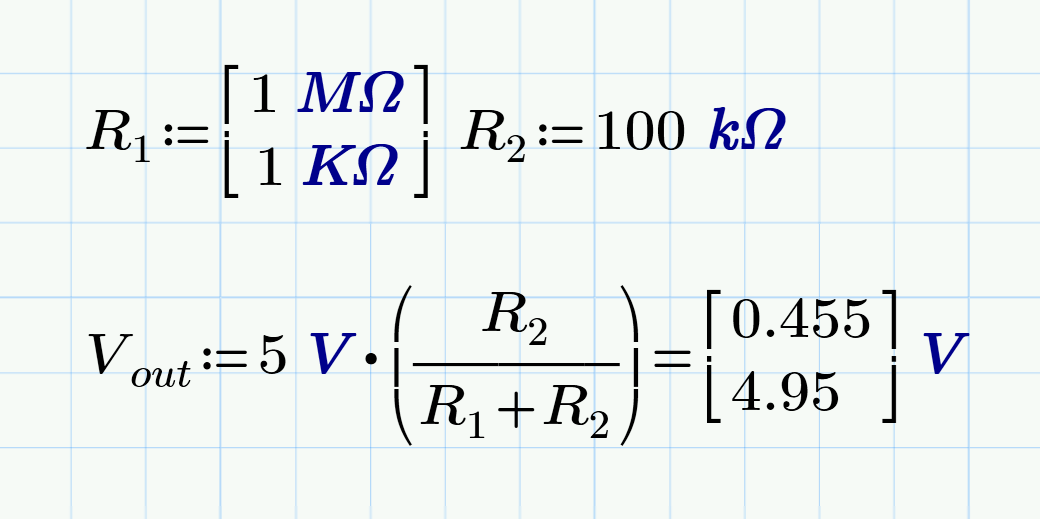
\includegraphics[scale=0.15]{Figure/FinalFormula.png}
\caption{Formula for a voltage divider with all known values and assumptions. Resulting in V\textsubscript{out} = 0.455V to 4.95V}
\label{fig:FinalFormula}
\end{figure}

The final circuit diagram, with all components included can be seen in \autoref{fig:Schematic2}. The blue boxes indicating which components should be on the shield it self, and where the Pin connector, connecting the shield to the glove should be.
\begin{figure}[H]
\centering
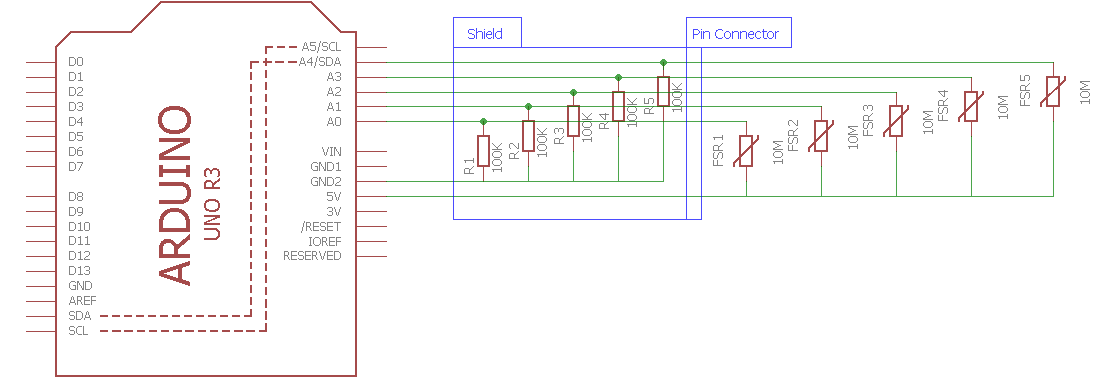
\includegraphics[scale=0.5]{Figure/Schematic2.png}
\caption{Schematic for the final circuit.}
\label{fig:Schematic2}
\end{figure}

The next step was to build an actual shield, seen in \autoref{fig:ShieldTopBottom} that would fit over the Arduino and connect to the sensors via a Pin connector. As this is just a prototype the shield was just made from a piece of through hole prototyping board cut down to a reasonable size and with pins soldered in on both sides to help get a solid connection with the Arduino.

\begin{figure}[H]
\centering
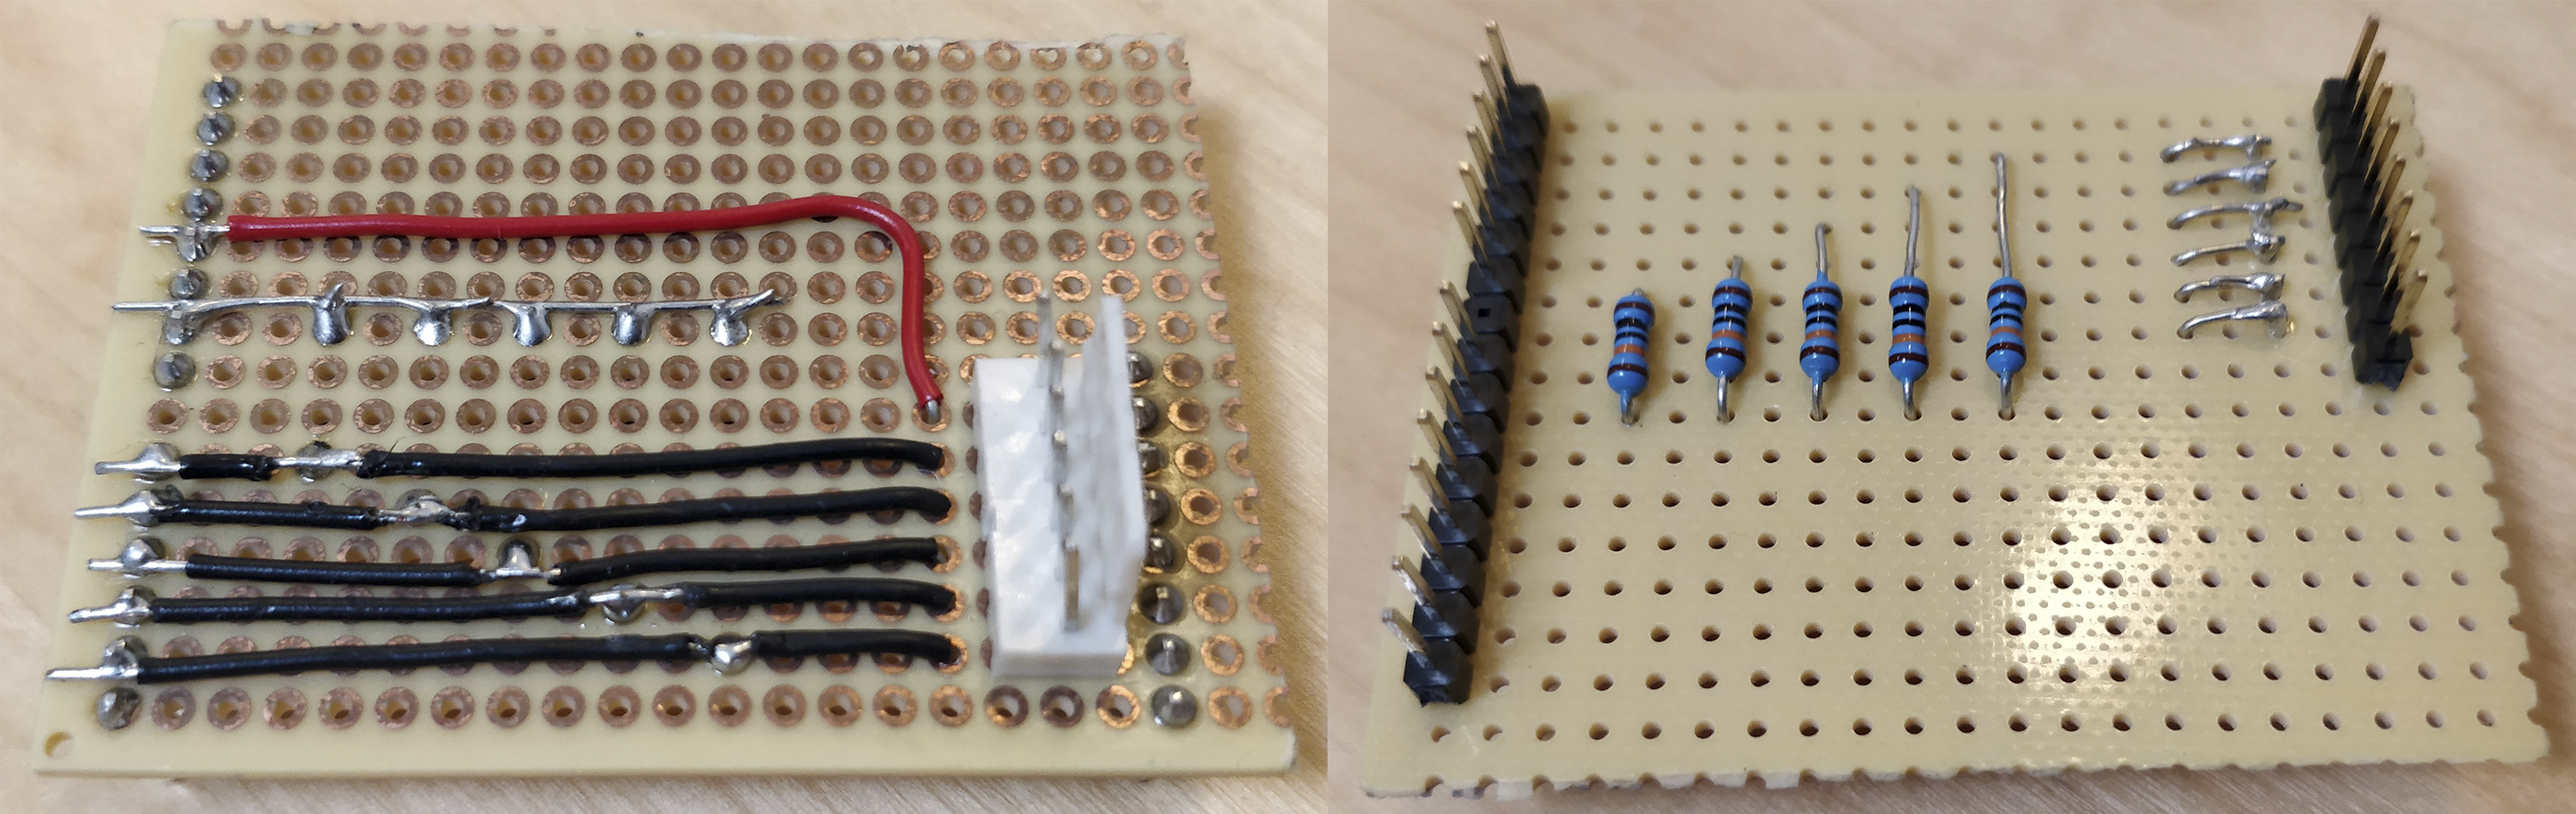
\includegraphics[scale=0.12]{Figure/ShieldTopBottom.png}
\caption{Picture of the actual shield. Left half is the top side of the shield and right half is the bottom. The Pin connector is the big white on the left half.}
\label{fig:ShieldTopBottom}
\end{figure}

The shield could also be made as a printed circuit board in which case it could look like \autoref{fig:TopBottomPCB}, here routed on both top and bottom side of the PCB in order to avoid collisions of paths and to maintain clarity.

\begin{figure}[H]
\centering
\includegraphics[scale=0.15]{Figure/TopBottomPCB.png}
\caption{An example of how the shield could be routed on PCB. Left is the top of the board, right is the bottom. PC\_6 is where the wires to the glove connect.}
\label{fig:TopBottomPCB}
\end{figure}
